%%%%%%%%%%%%%%%%%%%%%%%%%%%%%%%%%%%%%%%%%
% Template modified from:
% Programming/Coding Assignment
% LaTeX Template
%
% Original author of template:
% Ted Pavlic (http://www.tedpavlic.com)
%%%%%%%%%%%%%%%%%%%%%%%%%%%%%%%%%%%%%%%%%

% Original author of content:
% Paul Thrane
% Please feel free to copy/edit/distribute
% The author takes no responsibility for any mistakes that might be present.

%%%%%%%%%%%%%%%%%%%%%%%%%%%%%%%%%%%%%%%%%


%----------------------------------------------------------------------------------------
%	PACKAGES AND OTHER DOCUMENT CONFIGURATIONS
%----------------------------------------------------------------------------------------

\documentclass{article}

\usepackage{fancyhdr} % Required for custom headers
\usepackage{lastpage} % Required to determine the last page for the footer
\usepackage{extramarks} % Required for headers and footers
\usepackage[usenames,dvipsnames]{color} % Required for custom colors
\usepackage{graphicx} % Required to insert images
\usepackage{listings} % Required for insertion of code
\usepackage{courier} % Required for the courier font
\usepackage{hyperref} % Make references available
\usepackage{amsmath}

% Margins
\topmargin=-0.45in
\evensidemargin=0in
\oddsidemargin=0in
\textwidth=6.5in
\textheight=9.0in
\headsep=0.25in

\linespread{1.1} % Line spacing

% Set up the header and footer
\pagestyle{fancy}
\lhead{\sadTitle} % Top left header
%\chead{ } % Top center head
%\rhead{ } % Top right header
%\lfoot{ } % Bottom left footer
\cfoot{} % Bottom center footer
\rfoot{Page\ \thepage\ of\ \protect\pageref{LastPage}} % Bottom right footer
\renewcommand\headrulewidth{0.4pt} % Size of the header rule
\renewcommand\footrulewidth{0.4pt} % Size of the footer rule

%\setlength\parindent{0pt} % Removes all indentation from paragraphs

\newenvironment{allintypewriter}{\ttfamily}{\par}

%----------------------------------------------------------------------------------------
%	CODE INCLUSION CONFIGURATION
%----------------------------------------------------------------------------------------

\input{sadLanguageDef.txt} 	%Load part of SAD language defined in sadLanguageDef.ext

%----------------------------------------------------------------------------------------
%	NAME AND CLASS SECTION
%----------------------------------------------------------------------------------------

\newcommand{\sadTitle}{A SAD Introduction}
\newcommand{\sadDate}{June 2017}

% \sourceLocation is used to refer to where this paper with the accompanying other files,
% change this command if the files are moved or if it is used for another project elsewhere 
\newcommand{\sourceLocation}{\url{https://github.com/Vaagen/SADintro}}

%----------------------------------------------------------------------------------------
%	TITLE PAGE
%----------------------------------------------------------------------------------------

%\title{
%\vspace{2in}
%\textmd{\textbf{\hmwkClass:\ \hmwkTitle}}\\
%\normalsize\vspace{0.1in}\small{Due\ on\ \hmwkDueDate}\\
%\vspace{0.1in}\large{\textit{\hmwkClassInstructor\ \hmwkClassTime}}
%\vspace{3in}
%}

\title{\huge{An Introduction to Strategic Accelerator Design (SAD)}}

\author{\textbf{Paul Thrane}}
\date{
	\sadDate \\ \ \\ \ \\
	This document and accompanying source files can (soon) be found on\\
	\sourceLocation\\ \ \\
	SAD manual page: \url{https://hep-project-sad.web.cern.ch/SADHelp/SADHelp.html}
	}


%----------------------------------------------------------------------------------------

\begin{document}

\maketitle
A lot of help has been given by Katsunobu Oide and Demin Zhou.

\
\

\textbf{NOTE:} Should you spot any mistakes or have wishes for new sections/expansion of existing sections, don't hesitate to send an email to pcthrane@stud.ntnu.no; I'll try to help you as soon as I can.

%----------------------------------------------------------------------------------------
%	TABLE OF CONTENTS
%----------------------------------------------------------------------------------------

%\setcounter{tocdepth}{1} % Uncomment this line if you don't want subsections listed in the ToC

\newpage
\tableofcontents
\newpage

%----------------------------------------------------------------------------------------
%	Introduction
%----------------------------------------------------------------------------------------

\section{Introduction}
%
\textbf{Please note:} No SAD expert has yet read through this document, there might be (and most probably are) some mistakes in the text.

\subsection{About SAD}
Strategic Accelerator Design (SAD) is a computer code developed at the Japanese High Energy Accelerator Research Organization (KEK) since 1986. It is used in the design, commissioning and operation of several accelerators including J-PARC, KEKB and now SuperKEKB. It features specialized commands for easy definition of beamlines, optics matching, particle tracking and more, in combination with a Mathematica style programming interface.
%Sadly there is a lack of documentation for SAD, and therefore one often depends on seeking help from experienced users.

\subsection{Further resources}
This document is intended primarily as a quick starting guide to SAD. 
For the purpose of reference, 
\url{https://hep-project-sad.web.cern.ch/SADHelp/SADHelp.html} 
includes a list of many of the commands available in SAD, together with descriptions and some examples, and will be referred to as the SAD manual page in this document. The list is easiest to navigate using the search function of your browser. Another resource is the SAD home page, \url{http://acc-physics.kek.jp/SAD/}, the front page of which is shown in Figure~\ref{fig:sadHomePage}.


%As such, the structure is perhaps not the best for easy reference, although I will endeavor to make the structure as clear as possible.
%There are a few other resources available, most importantly the SAD home page: \url{http://acc-physics.kek.jp/SAD/} where you will find among other things a list of many of the commands available in SAD. This list is easiest to navigate using the search function of your browser. 
%Figure~\ref{fig:sadHomePage} points out where to find this list on the SAD home page.
% Mention Oide's presentation?




\begin{figure}[h]
	\begin{center}
	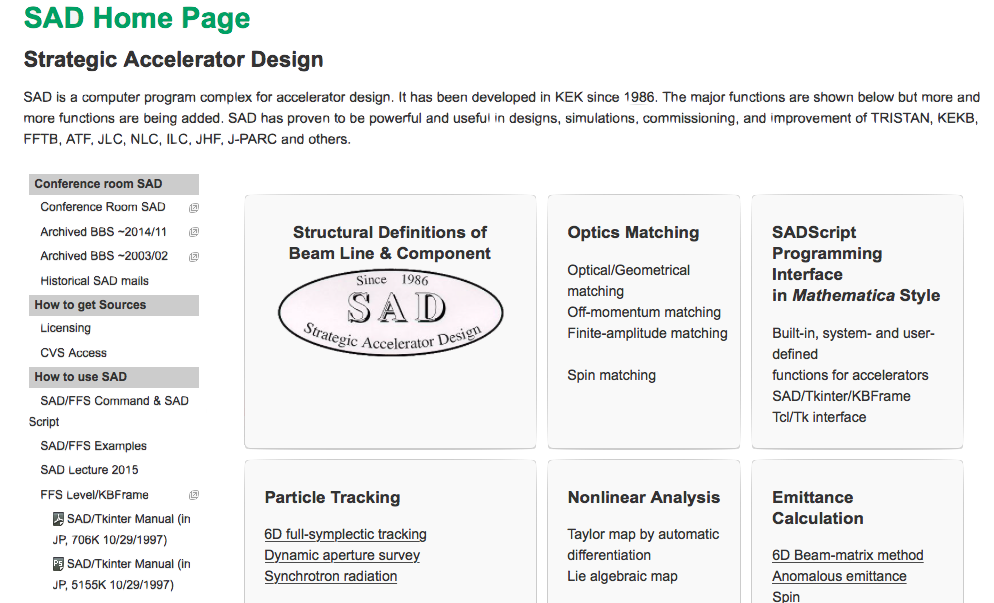
\includegraphics[width=0.75\columnwidth]{figures/sadHomePage.png}
	\end{center}
	\caption{Snapshot of the SAD home page, \url{http://acc-physics.kek.jp/SAD/}. The SAD Lecture 2015, by Katsunobu Oide, is also a good resource when starting out with SAD.}
	\label{fig:sadHomePage}
\end{figure}


\subsection{Installing SAD}
An up to date repository which includes brief installation instructions on Github: \url{https://github.com/KatsOide/SAD}.
Installing TCL/TK and X11 is recommended as this allows for using the graphical functions in SAD when e.g. plotting optical functions.

\clearpage

%----------------------------------------------------------------------------------------
%	Main Level
%----------------------------------------------------------------------------------------

\section{Main Level}
SAD is divided into two levels: the main level and the FFS level. Historically the FFS module was implemented to do optics matching for the final focus system in FFTB at SLAC.
% but has since then received many more functionalities. 
However, since then many more functionalities have been implemented in the FFS module. Some calculations and settings can be done in the main level, but since these can also be done in the FFS level they will not be mentioned here. The most important thing that has to be done while in the main level is the definition of lattice elements and the beamline.

As a brief note, commands in SAD are given on the form: %\texttt{COMMAND argument\_1 argument\_2 ...}
\begin{lstlisting}
COMMAND argument_1 argument_2 ...  ;
! While comments can be written behind an exclamation mark or between (*  *)
\end{lstlisting}
The command will take as many arguments as its definition allows unless terminated by a semicolon, thus it is recommended to end every command with \texttt{;} to make things clear.

\subsection{Defining a beamline}

\subsubsection{Elements}
Before we can start doing calculations with SAD we have to supply a model of an accelerator, which we will call a beamline.
The beamline is composed of elements representing magnets, monitors, cavities and other components that will affect the beam. To demonstrate how elements are defined, let us make two quadrupole magnets and two drift spaces, with the goal of later putting them together as a FODO cell.
%because there is nothing we would rather do than make a FODO cell
\begin{lstlisting}
DRIFT   L1=( L=1)   ! A drift space of length 1 m called L1.
        L2=( L=1)
;
QUAD    QF=( K1=0.75  L=0.5)   ! A horizontally focusing quadrupole magnet (K1>0)
        QD=( K1=-0.75 L=0.5)   ! Note: K1 is the integrated quadrupole field component
;
\end{lstlisting}
We have now defined two drift spaces of length 1 m called \texttt{L1} and \texttt{L2}. Also, we have defined two 0.5 m long quadrupole magnets with an integrated normal quadrupole field component \texttt{K1}$=gL/(B\rho)$ of 0.75 and -0.75 called \texttt{QF} and \texttt{QD} respectively, with $g$ as the field gradient and $L$ the magnet length. \texttt{K1}$>0$ means focusing in the horizontal plane (x-plane in the SAD coordinate system).
\par
Before we can define a beamline we also need at least one marker element to place at the beginning of the beamline. The reason is that SAD needs starting values for the optical functions to calculate the optics, and these should be defined in the first marker. If you wish to calculate optics with periodic conditions SAD will neglect these values when you turn on the RING flag (for periodic conditions), but the marker must be there when you define the beamline. The following code defines a marker element with transverse optical functions $\alpha_x=0$, $\alpha_y=0$, $\beta_x=5$ m and $\beta_y=3$ m, as well as a marker element without any predefined values. Such a marker may for example be used to later save optical function values at the end of the current beamline to be used to match the beginning of another beamline.
\begin{lstlisting}
MARK    START=( AX=0.0 AY=0.0 BX=5.0 BY=3.0)
        FINISH=()
;
\end{lstlisting}

Table~\ref{tab:elements} lists some of the available element types and accessible keywords. A more complete list and further explanations can be found on the SAD manual page.

\begin{table}[t]
	\begin{center}
	\caption{Some of the main element types. In addition to the mentioned keywords most elements also accept L, ROTATE, DX, DY, DISFRIN and DISRAD. More elements and keywords, as well as details can be found on the SAD manual page.}
	\label{tab:elements}
	\begin{tabular}[c]{lcl}
	Element		&	Some specific keywords		&	Comment				\\	\hline
	MARK		&	Optical functions, see Table \ref{tab:opticalFunctions}		 	&	Marker				\\
	DRIFT		&	L, RADIUS				&	Drift space			\\
	BEND		&	ANGLE, K0				&	Dipole magnet			\\
	QUAD		&	K1						&	Quadrupole magnet		\\
	SEXT		&	K2						&	Sextupole magnet		\\
	OCT 		&	K3						&	Octupole magnet		\\
	DECA		&	K4						&	Decapole magnet		\\
	DODECA		&	K5						&	Dodecapole magnet		\\
	MULT		&	K0 ... K21, SK0 ... SK21, BZ	&	Multipole magnet		\\
	SOL			&	BZ						&	Solenoid magnet		\\
	CAVI			&	VOLT, DVOLT, FREQ		&	RF cavity				\\
%	COORD		&							&	Coordinate transformation	\\
	APERT		&	AX,  AY					&	Aperture, for tracking		\\
	MONI		&							&	Monitor				\\
	BEAMBEAM	&							&	For beam-beam effect in tracking	\\
	MAP			& 	L						&	For user defined mapping, \\ & & \ \ look up ExternalMap on the SAD manual page \\
	\end{tabular}
	\end{center}
\end{table}

% Remember to use the fact that you will be doing examples, that is the main advantage of your approach!


%Key elements and their key properties, include some physics?

\subsubsection{Beamline}
With the previously defined elements we can now define a beamline that we call FODO:
\begin{lstlisting}
LINE    FODO=(START, QF, L1, QD, L2, FINISH)
;
\end{lstlisting}
We could also, for instance, make a beamline where we use one of the elements several times:
\begin{lstlisting}
LINE    FODOF=(START, QF, L1, QD, L2, QF, FINISH)
;    ! Note that QF appears twice
\end{lstlisting}
Here, using \texttt{QF} two times simulates a case where we have two quadrupole magnets connected to the same power supply; When matching they will have the same strength, while you can assign them different displacements or strength errors. They can be referred to separately as \texttt{QF.1} and \texttt{QF.2}. You are also allowed to use beamlines to define new beamlines:
\begin{lstlisting}
LINE    FODOF=(FODO, QF, FINISH)
;    ! Note here that we would also get two FINISH markers (there is one in FODO)
\end{lstlisting}
%
Furthermore, it is possible to invert the sequence of a beamline by using a minus(-), and repeat it $n$ times by using $n*$, like this:
\begin{lstlisting}
n=8;
LINE    ODOF=(-FODO)        ! The FODO cell in reverse order
        MANYFODO=(n*FODO)   ! A beamline of n FODO cells after each other
;
\end{lstlisting}

% markers and transport line
% Importing a lattice from another file

\subsubsection{Beam properties}
As mentioned, some optical functions can be given in the first marker. Other beam properties are stored in dedicated variables that can be accessed both from the main level and from FFS. Changing these variables can be done simply by assigning them the desired value.
\begin{lstlisting}
MOMENTUM=4e+9;    ! Nominal momentum at entrance of beamline in eV, here 4 GeV
PBUNCH=1e+10;     ! Number of particles in each bunch
MINCOUP=0.005;    ! Minimum emittance coupling EMITY/EMITX
\end{lstlisting}
Further variables defining the beam can be found on the SAD manual page. Note that by default, calculations in SAD are done assuming the positron mass and charge.




\clearpage
%----------------------------------------------------------------------------------------
%	FFS Level
%----------------------------------------------------------------------------------------

\section{FFS Level}
%The FFS module can be entered from the main level by the command \texttt{FFS;}, while single commands can be given to FFS by \texttt{FFS[" <command as string> "];}. To use a beamline
Before entering FFS the beamline must be defined, which for large lattices might be convenient to do in a separate file. To load such a file in the main level, you can use the \texttt{READ} command
\begin{lstlisting}
READ "myLatticeFileName.sad";
\end{lstlisting}
To subsequently enter the FFS module from the main level and choose a beamline to work with you use the \texttt{FFS} and \texttt{USE} commands, which may be combined to a single line:
\begin{lstlisting}
FFS USE FODO;
\end{lstlisting}
By default, the FFS command line parser converts input characters to uppercase, such that 
\begin{lstlisting}
ffs use fodo;
\end{lstlisting}
is equivalent to the previous example. This behavior can be changed by using the PRSVCASE flag.

\subsection{Calculating optics}
The optical functions are calculated using the command \texttt{CALCULATE}, which can be shortened by any number of letters down to \texttt{CAL}.
\begin{lstlisting}
CALC;
\end{lstlisting}
 The calculated values can then be accessed in several ways, such as by using
\begin{lstlisting}[mathescape=True]
result= Twiss["<optical function>","component"];
! For example:
by0= Twiss["BY","IP"]; ! $\color{ForestGreen}{\beta_y}$ at the component called IP is saved in by0
\end{lstlisting}
Note that optical functions are given at beginning of elements with finite length, contrary to e.g. the default behavior in MAD-X.

The closed orbit and equilibrium emittance is calculated using the \texttt{EMITTANCE} command, which similarly can be shortened to
\begin{lstlisting}
EMIT;
\end{lstlisting}


\subsection{Flags}
Many options for commands in SAD are set using flags. Table~\ref{tab:flags} lists some of the available flags, more flags and further details can be found on the SAD manual page.
Flags are set by simply writing the flag name. For example, to set periodic boundary conditions and calculate the resulting optical functions we would do
\begin{lstlisting}
CELL; ! Setting CELL flag
CALC; ! Calculating optics, with cell flag periodic boundary conditions are used
\end{lstlisting}
%
\begin{table}[h]
	\begin{center}
	\caption{Some of the flags available to set options in SAD. To turn off a flag you can add NO in front, for example NOCOD. Some flags have antonyms in addition, for example RING and TRPT.}
	\label{tab:flags}
	\begin{tabular}[c]{ll}
	Flag			&	Short description		\\	\hline
%	ABSW		&						\\
	CALC4D		&	Optical functions calculated using 4D plus dispersion, default.	\\
	CALC6D		&	Optical functions calculated using 6D.					\\
	CELL		&	Sets periodic conditions on calculation of optical functions.	\\
	COD			&	Closed orbit calculated when using EMITTANCE command.	\\
	CODPLOT	&	Closed orbit and extended Twiss parameters available using DISPLAY or DRAW commands.	\\
	EMIOUT		&	Extended output of EMITTANCE command.				\\
	FLUC		&	Enables the diffusion due to synchrotron radiation in the particle tracking.					\\
	GAUSS		&	Gaussian momentum distribution of the incoming beam, otherwise uniform.				\\
	GEOCAL		&	Geometry is updated when calculating optical functions, \\& \ \ turned off to e.g. simulate misalignments inside a solenoid.	\\
	INTRA		&	Includes intra beam scattering in emittance calculation.		\\
	RAD			&	Includes synchrotron radiation in particle tracking.			\\
	RADCOD		&	Includes energy loss due to synchrotron radiation for closed orbit calculation.				\\
	RFSW		&	Includes acceleration from cavities for tracking and emittance calculation.					\\
	TRPT		&	Transport line as apposed to ring, the nominal momentum can be changed along the beam line.\\
%				&						\\
%				&						\\
%				&						\\
%				&						\\
	\end{tabular}
	\end{center}
\end{table}

\subsection{Matching}
Matching can be done using the following commands,
\begin{lstlisting}
FIT <position>;
<Optical function> <goal value>;
FREE <element> <optional keyword>;
GO;
\end{lstlisting}
Table~\ref{tab:opticalFunctions} lists some of the available optical functions.
%
As an example, the periodic solution for the FODO lattice defined earlier has both a vertical and horizontal phase advance of 0.165121. If we want to change the quadrupole strengths such that the horizontal phase advance stays the same while increasing the vertical phase advance to 0.2147, for instance, we could execute the following code. The corresponding output from \texttt{GO} is shown in Figure~\ref{fig:goExample}.
%
\begin{lstlisting}[mathescape=true]
FIT FINISH;
NX 0.165121;   ! Setting goal value for horizontal phase advance
NY 0.2147;     ! Setting goal value for vertical phase advance
FREE Q*;       ! * is a wildcard that matches any combination of characters
               ! For other wildcards, see Table $\color{ForestGreen}{\ref{tab:wildcards}}$
! Above line is equivalent to: FREE Q* K1; as K1 is default keyword for quadrupoles
GO;            ! Starts the matching procedure
\end{lstlisting}
%
\begin{figure}[h]
	\begin{center}
	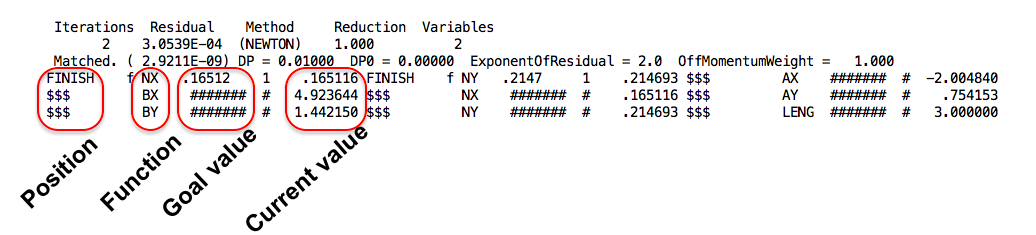
\includegraphics[width=1\columnwidth]{figures/goOutputExampleFODO.png}
	\end{center}
	\caption{Output example of \texttt{GO}. \$\$\$ is a special marker that points to the end of the beamline, while \textasciicircum \textasciicircum \textasciicircum \ points to the beginning.}
	\label{fig:goExample}
\end{figure}
%
Using the \texttt{VARIABLES} command, with short form \texttt{VAR}, we can list the changes to the variables, in this case K1 in QF and QD. The output is shown in Figure~\ref{fig:varExample}.
%
\begin{figure}[h]
	\begin{center}
	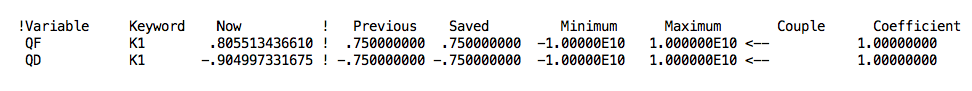
\includegraphics[width=1\columnwidth]{figures/varOutputExampleFODO.png}
	\end{center}
	\caption{Output example of \texttt{VAR}.}
	\label{fig:varExample}
\end{figure}

From Figure~\ref{fig:varExample} we can see that the new strength of QD is -0.9~m$^{-1}$, supposing that our quadrupole is limited to -0.85~m$^{-1}$ we could impose this constraint with the line
\begin{lstlisting}
QD MIN -0.85;    ! Upper limit can be set with MAX
! This method works for default keywords (K1 for quadrupoles)
\end{lstlisting}

A general expression can be fitted using \texttt{FitFunction}. To make an example of how this works, let us assume we have several dipole magnets called B1, B2, etc. and we want to free the bending angles of each individual magnet during the matching while still keeping the same total angle 
\begin{lstlisting}
originalTotalBendAngle = Plus@@LINE["ANGLE","B*"];
!Plus is a Mathematica function that sums terms, @@ applies Plus to the list from LINE
FitFunction:= Plus@@LINE["ANGLE","B*"] - originalTotalBendAngle;
FREE B* ANGLE;
<other matching conditions>
GO;
\end{lstlisting}
The matching procedure will try to make the value of \texttt{FitFunction} equal to zero, while also satisfying the other matching conditions.
To make an explicit dependance between two elements it is possible to use \texttt{ElementValues}:
\begin{lstlisting}
ElementValues = { key[elem] :> expr, ...};
\end{lstlisting}
For example,
\begin{lstlisting}
ElementValues = { "DY"["S1"] :> "DY"["S2"],  ! Setting DY of S1 equal to DY of S2
              "L"["D1"] :> "L"["D2"] *0.5};  ! Setting L of D1 equal to half L of D2
\end{lstlisting}
After matching variables can be made unfree by \texttt{FIX *}, while the matching conditions can be removed by \texttt{REJECT TOTAL}. Changes can be undone by using \texttt{RESET}, which removes changes made since the last call to \texttt{SAVE}.

\subsection{Matching Example}
I have not made this section yet; there is an official SAD example, but it would perhaps be good to have something similar here. Also, I have a cool MAX4 achromat that perhaps could be used. Send me an email ( pcthrane@stud.ntnu.no ) and I'll find the time to write something.

\subsection{Modifying the beamline in FFS}
Sometimes we wish to change the beamline we are working with, for example to remove or insert an element or to change which element comes first in a ring. This can be done using list manipulation functions. A few of these functions are \texttt{Insert}, \texttt{Delete}, \texttt{Drop}, \texttt{Take}, \texttt{Join}, \texttt{Prepend}, \texttt{Append}, whose behavior is equal to the corresponding functions in the Mathematica programming language (\url{http://reference.wolfram.com/language/}). In the following example we assume we have been working with a beamline and we now want to replace a drift called L1 with two shorter drifts, L2 and L3, including also a sextupole, S1, in between. We assume also that the new elements have been defined previously.
\begin{lstlisting}
BL=ExtractBeamLine[];         ! Extracting the current beamline and saving it as BL
L1pos=LINE["POSITION","L1"];  ! Getting the position of the drift we want to remove
BL2=Delete[BL,L1pos];
LSL=BeamLine[L2,S1,L3];       ! Making a new beamline segment to include 
BL2=Insert[BL2, LSL, L1pos];
USE BL2;                      ! Switching to the new beamline
\end{lstlisting}



%b=ExtractBeamLine[];
%b=Prepend[Drop[b,2],BeamLine[IP,BMBMP]];

%asc=ExtractBeamLine[];
%p=Position[asc,INJECTIO][[1,1]];
%asc1=Join[Take[asc,{p,-1}],Take[asc,{3,p-1}]];
%use asc1;

%Insert

%Append Complement Delete Depth Difference* Dimensions Drop Extract Flatten
 %  FlattenAt HeldPart Insert Intersection Join Length Part Partition Prepend
 %  Product Range ReplacePart Rest Reverse RotateLeft RotateRight Select 
 %  Sort Sum Take Table Union

%Example FODO

%Example CLIC FFS



%----------------------------------------------------------------------------------------
%	Output
%----------------------------------------------------------------------------------------

\section{Output}
\subsection{Write to file}
Writing to a file can be done by using \texttt{WriteString}. This can be used to for example save the calculated twiss values to a file for later use. Suppose we wish to save some twiss functions at the quadrupoles and monitors of a beamline.  After calculating the optics in SAD we can save the values to a file as follows, given that the quadrupoles are named with a Q first, while the monitors have a M first.
\begin{lstlisting}[mathescape=true]
pos=LINE["POSITION","Q*|M*"];	! Getting positions of elements starting with Q or M
fn=OpenWrite["twiss.out"];    ! Use OpenAppend[] if you do not wish to overwrite file
Do[                                    
 WriteString[fn, LINE["NAME",pos[i]] , "\t" , Twiss["BX",pos[i]] , "\t" ,               Twiss["BY",pos[i]] , "\n"]
 ! Here we write out $\color{ForestGreen}{\beta_x}$ and $\color{ForestGreen}{\beta_y}$
 ! For other optical functions, see Table $\color{ForestGreen}{\ref{tab:opticalFunctions}}$
 ,{i,Length[pos]}];
Close[fn];
\end{lstlisting}
Remember that the values are given at the beginning of components.
Note also that should you need to use a FFS function inside a Do-loop, e.g. \texttt{CALC} for recalculating optics, you must call it using the \texttt{FFS} function:
\begin{lstlisting}
FFS["CALC;"];
\end{lstlisting}


\subsection{Plotting}
I have not written anything about plotting yet. There is some info on the SAD home page. If you want me to add this section, send me an email ( pcthrane@stud.ntnu.no ) and I'll find the time.

%----------------------------------------------------------------------------------------
%	Tracking										       
%----------------------------------------------------------------------------------------

\section{Tracking}

\begin{lstlisting}
trackedBeam = TrackParticles[initialBeam, destination-component, nbegin, nend];
\end{lstlisting}
tracks the initial beam from rotation number \texttt{nbegin} to \texttt{destination-component} in rotation number \texttt{nend}. \texttt{nbegin} is increased by one when the beam is tracked past the end of the beam line and assumed to be 1 if it is not given. If \texttt{destination-component} is left out the tracking is done until the end of the beam line. The returned beam is of the same form as in the input, and is a list of the form
\\
\textbf{\{location, coordinates\}}
\\
Where location indicates the current position-number of the beam. The position-number can be acquired from the component name using \texttt{LINE["POSITION", "component-name"]}. The coordinates are of the form 
\\
\textbf{\{x, px/p0, y, py/p0, z, dp/p0, flag\}}
\\
with each term again being a list with length equal to the number of particles. Flag includes a value 1 or 0 for each particle, indicating if the particle is still in the ring (1), or if it is lost (0).
Further details can be found on the SAD manual page.

%Tracking is done using a function called \texttt{TrackParticles[]}, the following is 
%\textit{from the SAD home page} (~\url{http://acc-physics.kek.jp/SAD/}~):
%\begin{lstlisting}
%trackedBeam = TrackParticles[initialBeam, destination-component, nbegin, nend];
%\end{lstlisting}
%returns a beam after the tracking at the entrance of the destination-
%component. The destination can be specified by the name of the component
%or by a number obtained by \texttt{LINE["POSITION", component]}.   
%If destination is omitted, the end of the line is assumed.
%\\
%The argument nbegin is the initial turn number to be passed to tracking to indicate
%it is in the n-th turn. The number is increased by 1 when it passes the end of beam line.
%If nbegin is omitted, 1 is assumed.
%
%The argument nend is the last turn number. The default is nbegin.
%
%The variable beam and also the result of TrackParticles are lists of the
%form 
%\\
%   \{location, coordinates\}
%\\\
%where location is the position-number of the starting point.  If location is
%same as or in the downstream of destination, the tracking is done by 
%folding across the beginning of the beam line. The coordinates are in a list of {7, np}
%form, where np is the number of particles. The first 6 elements of
%coordinates specifies
%
%   \{x, px/p0, y, py/p0, z, dp/p0\}
%
%in this order.   The \{7, i\} is the flag which is True(==1) when the 
%particle is alive, and False(==0) when lost.
%
%   When a flag RADLIGHT is on, TrackParticles returns the trajectories of
%particles which are used to calculate the radiation fields.   See
%RadiationField and RadiationSpectrum.
%
%When PHOTONS is ON (default is OFF), TrackParticles generates a list of all
%photons radiated through the tracking. The list is assigned to a symbol PhotonList.

%%%%%%%%%%
\subsection{Tracking example}
Below is a general example of tracking in SAD, based on a script from Demin Zhou. More detailed examples, including a sample on how one can do statistics on the tracked beam are included together with the source code for this text at \sourceLocation
\lstinputlisting{"sadCode/minimalTrackingExample.sad"}


%Tracking is done using a function called \texttt{TrackParticles[]}, with the arguments
%\begin{lstlisting}
%TrackParticles[beam, destination-component, nbegin, nend];
%\end{lstlisting}
%The beam variable is of the same format as the returned result, and stores the 
%\{location , \{ x , y , z \} \} 

%%%%%%%%%%
\subsection{Comments on statistical calculations during tracking}
Here are a few practical notes regarding doing statistics on a tracked particle beam in SAD. First is an example of how the mean and variance can be calculated from the beam variable, in addition to fitting a Gaussian distribution to the tracked particles. 

\begin{lstlisting}
! variables for saving mean and variance should be defined before starting tracking
 xave=Table[0,{i,7}];
 x2ave=Table[0,{i,7}];

! Then, during tracking, they can be calculated ...
! ... by RMS:
xave=Plus@@[pbeam,{1}]/np;
x2ave=Plus@@[(pbeam-xave)^2,{1}]/np;
! here, x2ave is the variance

! ... by fitting to a Gaussian distribution:
 Do[
    fdp = fd@FitGaussian[pbeam[[k]],Plot->False];
    ! FitGaussian not part of SAD functions, must be defined, see below
    xave[[k]] = fdp[[2]];
    x2ave[[k]] = fdp[[1]],
    ! here, if FitGaussian is implemented as below, x2ave is the standard deviation
    {k,6}];
! The different coordinates can then be accessed using ave[[1]], ... ave[[6]]
\end{lstlisting}
Note that to fit the particles to a Gaussian distribution you must have previously defined a fitting function, for example:
\lstinputlisting{sadCode/fitGaussian.sad}

If you have particles getting lost their coordinates may become arbitrary large, messing up the statistical calculations and possibly causing errors that stop your code. A simple solution is to use the survival flag to identify any lost particles and remove them:
\lstinputlisting{sadCode/deleteParticleFromBeam.sad}

%%%%%%%%%%
\subsection{Dynamic aperture}
The dynamic aperture can be calculated using the function
\begin{lstlisting}
DynamicApertureSurvey[range, nturn, options];
\end{lstlisting}
which does single particle tracking for \texttt{nturn} number of turns for particles distributed evenly within \texttt{range}.
The range is a list \{xrange, yrange, zrange\} with xrange equal to \{xmin, xmax\} and similarly for yrange. zrange is a list containing all the desired z values to calculate the dynamic aperture for. All the range values are the initial amplitudes divided by the equilibrium values calculated by the \texttt{EMITTANCE} command. For each z value, 51 x and y values are chosen linearly spaced in the corresponding ranges. Some of the available options are listed on the SAD manual page, and include the possibility to choose between x, y or z as the axis where you specify the values, as well as the possibility to change the starting phase of the particles in e.g. the (x,px) phase space. The ensuing code is an example of how one may call \texttt{DynamicApertureSurvey} for the SuperKEKB Low Energy Ring, followed by the resulting output.
%
\lstinputlisting{sadCode/dynamicApertSurveyExample.sad}
%
\begin{figure}[h]
	\begin{center}
	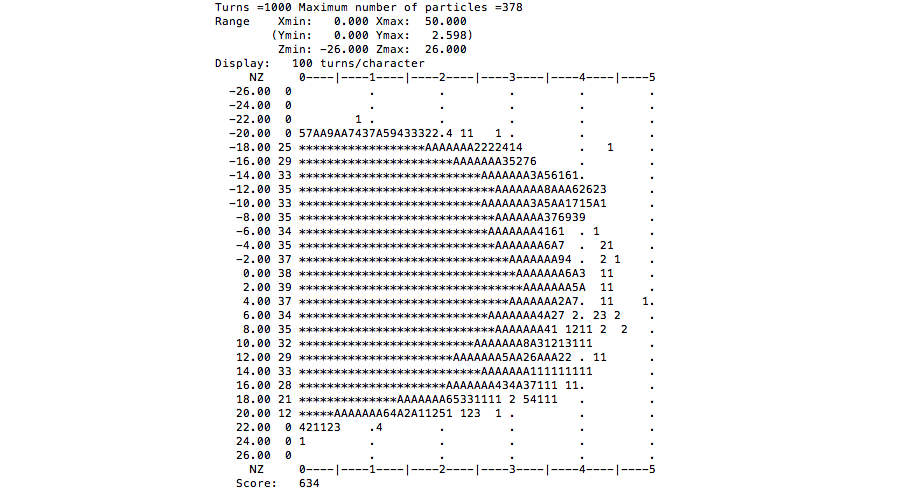
\includegraphics[width=1\columnwidth]{figures/dynamicApertSurveyOutput.png}
	\end{center}
	\caption{Output example of \texttt{DynamicApertureSurvey[]} for the code above. An "A" means the particle survived all turns of the tracking, while "\texttt{*}" means the particle has not been tracked but is assumed to survive. The number of survived particles before the rest are assumed to survive can be changed in the variable DAPWIDTH (default 7). More details can be found on the SAD manual page.}
	\label{fig:dynamicApertSurveyOutput}
\end{figure}



%%%%%%%%%%
\subsection{Beam-beam effect and luminosity}
When tracking it is possible to include the beam-beam effect from a colliding beam using the \texttt{BEAMBEAM} element, here defined for the SuperKEKB Low Energy Ring
\begin{lstlisting}
 BEAMBEAM    BMBMP  =(NP=6.53E10 BETAX=0.025 BETAY=0.0003 EX=0.0
             EY=0.0 EMIX=4.6E-9 EMIY=12.88E-12 DP=6.37E-4 
             ALPHAX=0.0 ALPHAY=0.0 SIGZ=5.0E-3 DX=0.0 DZ=0.0
             SLICE=200.0  XANGLE=41.5E-3 STURN=1000)
; ! The arguments describe the colliding beam, which is not affected by the tracking
\end{lstlisting}
When tracking the beam through a \texttt{BEAMBEAM} component, the luminosity is calculated and sent to a virtual function called \texttt{LuminosityMonitor[]}. By defining this function you can obtain the calculated value and for example save it to a variable 
\begin{lstlisting}
! Before tracking: initializing an empty table and defining LuminosityMonitor
LumTab={};
LuminosityMonitor[lum_]:= (LumTab=Append[LumTab,lum];);
\end{lstlisting}
The luminosity sent to \texttt{LuminosityMonitor[]} is
\begin{equation*}
L_{SAD}=\frac{\mathcal{L}}{f_0N_bN_1N_2},
\end{equation*}
where $\mathcal{L}$ is the luminosity in m$^{-2}$s$^{-1}$, $f_0$ is the revolution frequency and $N_b$ the number of bunches. $N_1$ and $N_2$ are the number of particles per bunch in each of the two beams.

%----------------------------------------------------------------------------------------
%	Control Structures  - Should be underneath Mathematica basics if included
%----------------------------------------------------------------------------------------

%\section{Flow-control}
%Do\\
%If\\
%While\\
%For\\
%Use FFS["...;"];\\

%----------------------------------------------------------------------------------------
%	Adding errors
%----------------------------------------------------------------------------------------

\section{Adding errors}
Suppose we want to introduce errors to our lattice for some study. The following example shows how to do this for all the quadrupoles in a beamline assuming their names start with Q (so that they are matched by the wildcard Q*). For a list of available wildcards see Table~\ref{tab:wildcards}. Notice the $+=$, with only $=$ you will replace the original value with the error instead of adding them.
\begin{lstlisting}[mathescape=true]
sigmaX= 1e-4;     ! A temporary variable for standard deviation in x, here 100 $\color{ForestGreen}{\mu}$m
sigmaY= 1e-4;
sigmaROT= 1.5e-4; ! For standard deviation in rotation, here 150 $\color{ForestGreen}{\mu}$rad
sigmaK= 8e-4;     ! For standard deviation in strength, here 0.08%
SeedRandom[2];    ! Seeding the pseudo random-number generator
Qpos=LINE["POSITION","Q*"];    ! Saving quadrupole positions
LINE["DX",Qpos]     += GaussRandom[Length[Qpos]]*sigmaX;
LINE["DY",Qpos]     += GaussRandom[Length[Qpos]]*sigmaY;
LINE["ROTATE",Qpos] += GaussRandom[Length[Qpos]]*sigmaROT;
LINE["K1",Qpos]     += GaussRandom[Length[Qpos]]*sigmaK;
CALC;             ! Remember to run CALC to recalculate optics
\end{lstlisting}

%----------------------------------------------------------------------------------------
%	Wildcards
%----------------------------------------------------------------------------------------

\section{Wildcards}
Table~\ref{tab:wildcards} lists wildcards available in SAD.
\begin{table}[h]
	\begin{center}
	\caption{Wildcards in SAD. Can be used to select several components without explicitly listing every one.}
	\label{tab:wildcards}
	\begin{tabular}[c]{cl}
	Wildcard			&	Short description								\\	\hline
	*				&	Matches any sequence of characters (including none).	\\
	\{...\}				&	Matches any single character inside \{\}.				\\
	\{\textasciicircum ...\}	&	Matches any single character except those inside \{\}.	\\
	\%				&	Matches any single character.						\\
	a$|$b$|$...		&	Matches a or b or ...								\\
	\end{tabular}
	\end{center}
\end{table}

%----------------------------------------------------------------------------------------
%	Optical functions
%----------------------------------------------------------------------------------------

\section{Optical functions}
Table~\ref{tab:opticalFunctions} lists some of the optical functions available in SAD. They can be calculated and updated using the \texttt{CALC} command, and can be accessed by using the \texttt{DISPLAY} command or the \texttt{Twiss[]} function.
\begin{table}[h]
	\begin{center}
	\caption{Some of the optical functions in SAD. }
	\label{tab:opticalFunctions}
	\begin{tabular}[c]{cl}
	Function		&	Short description								\\	\hline
	AX , AY		&	$\alpha_x$,  $\alpha_y$			\\
	BX, BY		&	$\beta_x$, $\beta_y$				\\
	NX, NY		&	$\psi_x$, $\psi_y$, transverse phase advance	\\
	EX, EY		&	$\eta_x$, $\eta_y$, transverse dispersion		\\
	EPX, EPY		&								\\
	R1			&								\\
	R2			&								\\
	R3			&								\\
	R4			&								\\
	DX, DY		&	$\Delta x$, $\Delta y$			\\
	DPX,	 DPY		&								\\
	DDP			&	$\Delta p /p_0$					\\
	AZ			&	$\alpha_z$					\\
	BZ			&	$\beta_z$						\\
	NZ			&	$\psi_z$, longitudinal phase advance	\\
	TRX, TRY		&	Trace($T_x$), Trace($T_y$), defined for end of beamline		\\
	LENG		&	Length of design orbit			\\
	\end{tabular}
	\end{center}
\end{table}


%AX      alpha_X
%BX      beta_X
%NX      psi_X, the default scale is 1/(2Pi)
%AY      alpha_Y
%BY      beta_Y
%NY      psi_Y, the default scale is 1/(2Pi)
%EX      eta_X   (dispersion_X)
%EPX     eta_Px  (dispersion_PX) 
%EY      eta_Y   (dispersion_Y)
%EPY     eta_Py  (dispersion_PY)
%R1      R_1     (see x-y-coupling)
%R2      R_2     (see x-y-coupling)
%R3      R_3     (see x-y-coupling)
%R4      R_4     (see x-y-coupling)
%DETR    R_1*R_4 - R_2*R_3 (see x-y-coupling)
%DX      dx
%DPX     dpx
%DY      dy
%DPY     dpy
%DZ      dz
%DDP     delta=dp/p0
%AZ      alpha_Z
%BZ      beta_Z
%NZ      psi_Z, the default scale is 1/(2Pi)
%ZX      zeta_X  (z-dispersion_X)
%ZPX     zeta_Px (z-dispersion_PX) 
%ZY      zeta_Y  (z-dispersion_Y)
%ZPY     zeta_Py (z-dispersion_PY)
%PEX     eta_x   (dispersion_x)
%PEPX    eta_px  (dispersion_px) 
%PEY     eta_y   (dispersion_y)
%PEPY    eta_yy  (dispersion_py)
%TRX     trace(T_X), only defined at the end of the beam line.
%TRY     trace(T_Y), only defined at the end of the beam line.
%LENG    length of the design orbit

%----------------------------------------------------------------------------------------
%	Mathematica basics
%----------------------------------------------------------------------------------------

\section{Mathematica basics}
I have not written anything about Mathematica basics yet. If you want me to add this section, send me an email ( pcthrane@stud.ntnu.no ) and I'll find the time.

%Include Mathematica basics and SAD peculiarities? \\
%Scoping for example

%----------------------------------------------------------------------------------------
%	comments
%----------------------------------------------------------------------------------------

%\section{Stuff still in need of a place}
%Wildcards\\
%FODO example\\
%CLIC FFS example\\
%Importing another file\\
%Table of optical function names\\
%BEAM-BEAM element\\
%Luminosity calculation\\
%DynamicApertureSurvey\\
%accessing element values, LINE\\
%DISFRIN\\
%Values at end of elements\\
%Logical operators\\
%Do loop and If structure\\
%Calculating emittance\\
%$<=>$ as NOT\\
%Translation of lattices\\
%Defining functions, Mathematica style\\
%GET[]\\
%
%Optimizing using DownhillSimplex?\\
%
%
%end;
%
%GEO; in errors?

%----------------------------------------------------------------------------------------
%	comments
%----------------------------------------------------------------------------------------

%\section{temporary: formating code in \LaTeX}
%
%If you want to name a function inside text, use $\backslash$texttt\{calc;\} to write  \texttt{calc;}.
%
%$\backslash$ lstinputlisting\{sadCode.sad\}
%
%$\backslash$ begin\{lstlisting\} ... $\backslash$ end...
%\begin{lstlisting}
%FFS;
%!do some sad stuff
%end;
%\end{lstlisting}
%
%\begin{figure}[h]
%	\begin{center}
%	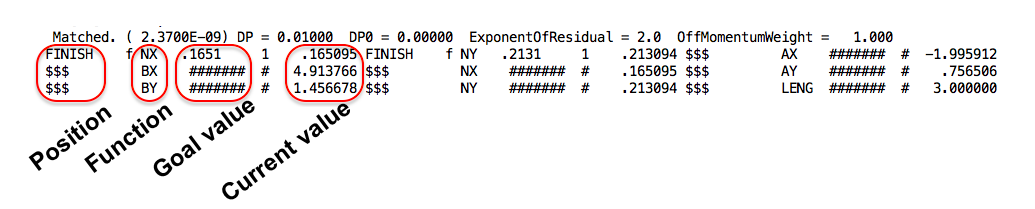
\includegraphics[width=1\columnwidth]{figures/calcOutputExampleFODO.png}
%	\end{center}
%	\caption{Output example of CALC. \$\$\$ is a special marker that points to the end of the beamline, \textasciicircum \textasciicircum \textasciicircum \ points to the beginning.}
%	\label{fig:calcExample}
%\end{figure}



%----------------------------------------------------------------------------------------

\end{document}